\documentclass[sigconf]{acmart}

\settopmatter{printacmref=false} % Removes citation information below abstract
\renewcommand\footnotetextcopyrightpermission[1]{} % removes footnote with conference information in first column
\pagestyle{plain} % removes running headers

\usepackage{booktabs} % For formal tables


% Copyright
%\setcopyright{none}
%\setcopyright{acmcopyright}
%\setcopyright{acmlicensed}
\setcopyright{rightsretained}
%\setcopyright{usgov}
%\setcopyright{usgovmixed}
%\setcopyright{cagov}
%\setcopyright{cagovmixed}
\usepackage{graphicx}

\copyrightyear{2017}


\acmArticle{4}
\acmPrice{15.00}


\begin{document}
\title{TrailBlazer - Final Report}
\subtitle{CSE6242 FALL2017}


\author{\textbf{Alexandre Palo}}
\affiliation{%Chamb\'{e}ry
  \institution{Georgia Institute Of Technology}
  \streetaddress{North Avenue}
  \city{Atlanta} 
  \state{Georgia} 
  \postcode{30332}
}
\affiliation{%
  \institution{\'{E}cole nationale sup\'{e}rieure d'arts et m\'{e}tiers}
  \streetaddress{151 Boulevard de l'Hôpital}
  \city{Paris} 
  \state{France} 
  \postcode{75013}
}
\email{alexandre.palo@gatech.edu}

\author{\textbf{Guillaume Broggi}}
\affiliation{%
  \institution{Georgia Institute Of Technology}
  \streetaddress{North Avenue}
  \city{Atlanta} 
  \state{Georgia} 
  \postcode{30332}
}
\affiliation{%
  \institution{\'{E}cole nationale sup\'{e}rieure d'arts et m\'{e}tiers}
  \streetaddress{151 Boulevard de l'Hôpital}
  \city{Paris} 
  \state{France} 
  \postcode{75013}
}
\email{guillaume.broggi@gatech.edu}

\author{\textbf{Alex Mueller}}
\affiliation{%
  \institution{Georgia Institute Of Technology}
  \streetaddress{North Avenue}
  \city{Atlanta} 
  \state{Georgia} 
  \postcode{30332}
}
\email{alex.mueller@gatech.edu}

\author{\textbf{Tianyi Zheng}}
\affiliation{%
  \institution{Georgia Institute Of Technology}
  \streetaddress{North Avenue}
  \city{Atlanta} 
  \state{Georgia} 
  \postcode{30332}
}
\email{tianyi.zheng@gatech.edu}

\maketitle

\section{Introduction}

Right now there is no convenient web application to help bikers and hikers find enjoyable trails. The best option is something like Google Maps, but it is designed to go from a point A to a point B and it lacks crucial meta-information like trail conditions and difficulty. In order to find this information, users have to refer to additional websites which further complicates the process. Additionally, Google Maps does not have points of interest (POI) that are geared towards hikers. Our goal is to create an application that not only helps bikers and hikers find trails but to also introduce them to unique and interesting POI that would not have seen otherwise.

\section{Related work}
Because there is no all-in-one application that do exactly what we plan to do, there is little previous literature regarding similar applications. However, there is plenty of literature surrounding our project's component parts: data, database, backend, and user-interface.

All of our data is either open-source or crowd-sourced. This leads to our major risks: users getting lost or injured. Our map data is pulled from OpenStreetMap, which according to Haklay, has fairly impressive coverage. However, it is somewhat lacking in low-population areas (Haklay 2010). This could cause issues with finding accurate trail data. Our trail quality/difficulty and POI information are pulled from crowdsourcing sites that may have issues in information quality. One possible solution is to look at user reviews to determine data quality so that we can filter out low quality data (Allahbakhsh 2013).

As for the database, Amirian, et al. compared the performance and scalability of SQL databases, spatial databases (SQL with support for spatial data), and an XML document NoSQL database. NoSQL showed better performance in single and multiple geospatial feature retrieval queries (Amirian, et al. 2014). Agarwal, et al. also ran geospatial querying tests specifically comparing MongoDB and PostgreSQL (with PostGIS) databases. They found MongoDB performed on average 10 times better than PostgreSQL with PostGIS (Agarwal 2017). Additionally, MongoDB's document structure makes it perfect for GeoJSON.

We use the REST API for our backend, implemented by a Django Python server. In a REST API, the frontend is independent from the stateless backend. The backend also has a uniform data interface which is implemented such that it will respond to any request with minimal information from the client (Fielding 2000).

The most promising algorithms for path generation were from Tarjan and Johnson. Tarjan outlined an algorithm that uses Dijkstra's algorithm to find the shortest path between nodes and uses depth-first search to find cycles/blocks that can be used as paths (Dijkstra 1959, Tarjan 1972). Johnson also designed an algorithm that finds all simple cycles in a directed graph (Johnson 1975). We instead chose to implement a very simple algorithm, based on a computed weight for each node. The major challenge is then to build a tree based on OpenStreetMap roads.

In order to develop an effective UI, Rosenzweig says that we need to know the demographics of our users as well as how they will use our application. By investigating the use cases for our application, we can ensure that the the UX is as smooth as possible to our users (Rosenzweig 2015). Thus, we used several iterations to select the best UI for our application (See figure \ref{table:ux_iterations}).

\section{Proposed method}
In order to generate an ideal path, we propose a method of weighting nodes of a graph to direct algorithmic path generation. These weights will be based on proximity to points of interest and preexisting outdoor trails.

\begin{table}
    \begin{tabular}{|lrrr|}
         \hline
         & & & Iterations \\
         & 1 & 2 & 3 \\
         \hline
         Guillaume Broggi & 5.0 & 7.5 & 8.0
         \\
         Alexandre Palo & 7.0 & 8.0 & 10.0
         \\
       	 Alex Mueller & 4.5 & 6.5 & 9.0
       	 \\
       	 Tianyi Zheng & 5.0 & 7.0 & 8.5
       	 \\
         \hline
         Average & 5.34 & 7.25 & 8.88
         \\
         \hline
    \end{tabular}
    \captionsetup{justification=centering}
    \caption{UX iterations.}
    \label{table:ux_iterations}
\end{table}

\subsection{Data collection and processing}
Our weighting data came from two websites: utagawavtt.com and geocaching.com. Utagawa lists crowd-sourced mountain bike trails in France, and Geocaching provides crowd-sourced points of interest. Neither website had a public API, so we had to scrape the data. Scraping data from utagawavtt.com was fairly straightforward, and we designed a script that utilized the website's search functionality. In order to scrape data from geocaching.com, we first needed to extract the POI IDs, and then we used the IDs to find their respective pages where we could extract data. Scraping all of the POI within France took over 250,000 HTTP requests and approximately 14 hours to complete.

This data was used to generate POI proximity weight (poiWeight) and Utagawa proximity weight (trackWeight) for the nodes in our trails, which were pulled from OpenStreetMap, which was downloaded from Mapzen's metro extracts. We chose OpenStreetMap to be the base of our system because of its generally good coverage (Haklay 2010). Additionally, we filtered out major highways and busy roads from our OpenStreetMap data set in order to ensure that users would not be directed into dangerous situations. This data was all stored in a MongoDB database hosted by MongoDB's Atlas service.

PoiWeight corresponds to the proximity of a node to points of interest from geocaching.com. This value was computed by searching for all trails within a 1 km radius of each POI. For each of these trail, we found the trail nodes that were contained in the radius and incremented their individual poiWeight attribute by $2 -d$, where $d$ is the distance between the POI and the trail node.

\begin{figure}[htbp]
  \centering
  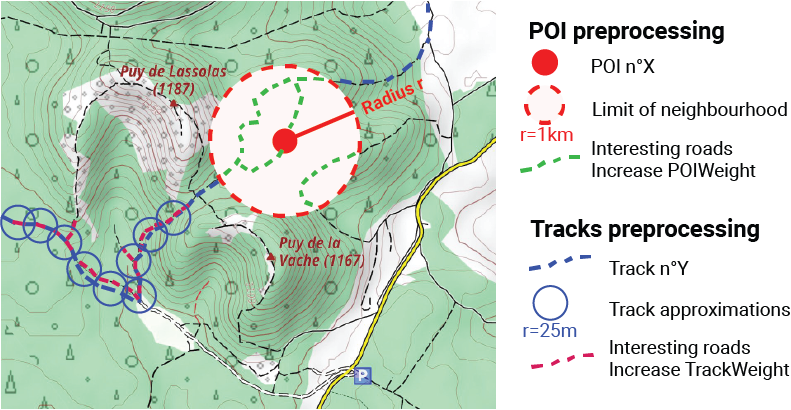
\includegraphics[width=\columnwidth]{prepro.png}
  \caption{Preprocessing data to populate OpenStreetMap}
\end{figure}

TrackWeight was computed similarly. The nodes on Utagawa trails are collected from a contributor's personal GPS system, so we cannot guarantee that trails from Utagawa completely match up with the trails on OpenStreetMap. Wing, et al. found that consumer GPS systems were had errors ranging from 3 m to 7 m, so if a Utagawa trail is at most 25 m away from an OpenStreetMap trail, we assume that they are the same trail (Wing 2005). We computed a bounding box for each Utagawa trail in our database and used MongoDB geospatial queries to find all OpenStreetMap trails that were within or intersect the bounding box. We then iterated through the nodes each of these OpenStreetMap trails, and if the node was within 25 m of the Utagawa trail, its trackWeight attribute was incremented by 1. 

This pre-processing was computationally-intensive, but it reduced the amount of processing needed when running our application. After processing, the dataset used by our application consisted of a sampling of OpenStreetMap nodes and edges, where each node had been weighted for POI and Utagawa trail proximity. In total, we collected and processed 11,130 Utagawa trails, 246,984 geocache POI, and 354,883 roads from OpenStreetMap.

\subsection{Processing based on user inputs}

Users select their start point on a map in an online interface built with the JavaScript library React from Facebook. These points will be passed to a backend REST API that was implemented using Python and Django. The backend application queries every node within a circle whose radius corresponds to the maximum distance chosen by the user. Then, the application then uses the networkx Python library to build a graph using these nodes and the edges that link them.

When the graph is built, the algorithm searches for paths by maximizing the weight of the overall path. The weight used is a combination of poiWeight and trackWeight, balanced with user preferences:

\begin{equation}
	weight = a*poiWeight + b*trackWeight
\end{equation}
\begin{equation}
	(a, b) \in [0, 10]
\end{equation}
where $a$ and $b$ represent preference for trails or POIs, respectively. Both are provided by the user via the front-end interface. 

The path finding algorithm works similarly to the Dijkstra's shortest path method. It uses a naive approach to always pick the highest overall weighted edge and traverses the graph starting from the initial location. It never takes the same edge twice, unless it reaches a dead end and then it traverses backwards. It also marks nodes as unfinished when the node has still has untraveled out-going edges in order to improve performance. The algorithm traverses until it reaches the desired length. This operation is performed for several iterations, and the paths with the top overall weights are chosen.

\begin{figure}[htbp]
  \centering
  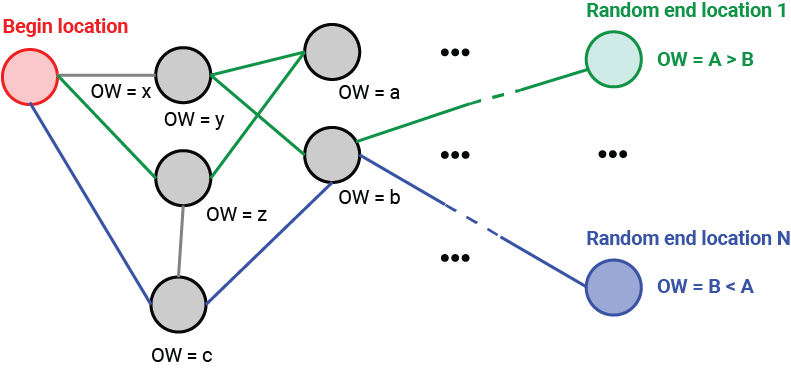
\includegraphics[width=\columnwidth]{pro.png}
  \caption{Processing graph algorithm}
\end{figure}

When the algorithm finishes running, it sends results to the React front end application in the form of a json file. The number of results sent to the front end is dependent upon how many heavily weighted trails the algorithm produces. For example, if the start point is in a forest, there may only be a small number of possible paths because there are far fewer roads and trails for the algorithm to traverse.

% there may only be a small number of possible paths if the start point 

% The algorithm can return a single solution with the largest weight or an array or two or more solutions 

% It can be a single solution based on the best weight it found, or an array of two or more solutions when a lot of solutions were possible during the computation. For instance, in the forest, only a small number of roads exist and the number of road junctions is limited and a lot smaller than in the main city.

\subsection{Displaying results}
The UI application displays the results as interactive paths on a map. Users can select a path on the map and view information about locations along the path via a bar graph that shows the current point on the path. The application also displays useful information such as the average poiWeight and trackWeight and path length to help the users asses the quality and usefulness of the path.

% results on a map to let the user see the real path of the solution. Moreover, it let the user select the solution he was to see on the map and browse it thanks to a bar graph showing the current point of the track. The application also display useful information to assess the quality and the usefulness of the solution proposed like the average value of poiWeight or trackWeight, and the total distance of the track.

To finish, a button lets the user download the selected track in the GPX file format. This format is useful because it is the standard format for map application and GPS devices. It will let the user follow this track on his bike afterward for instance. After all, going outside is the aim of the application.

\subsection{Front end mechanism}
In order to display useful information (example of interface in the figure \ref{figure:ux}), gather user input, and send requests to the server, we used Facebook's open source JavaScript library React. This library was useful for creating a "one page" application only in JavaScript and has a lot of advantages against "heroic" JavaScript (without any framework) and other libraries such as Vue.js or Angular:

\begin{itemize}
\item The React library lets us create components for our application and encourages us to reuse them. For instance, we create a "Track" component which correspond the a track displayed on the Map. All the behaviors a component (hover event, display behavior, ...) are only coded once and are easily changed thanks to this framework.
\item Every time the state of the application changes, the framework computes the next state of each component. However, it is coded such that the only component that have really changed are re-rendered on the screen. Thus, the application is fast and has good performance.
\item We used React with Webpack, a JavaScript module bundler for the web, Babel, and NodeJS. NodeJS let us to easily use other existing library and Babel to write JavaScript with the latest version ES2015, which is very convenient.
\end{itemize}

\begin{figure*}
  %\centering
  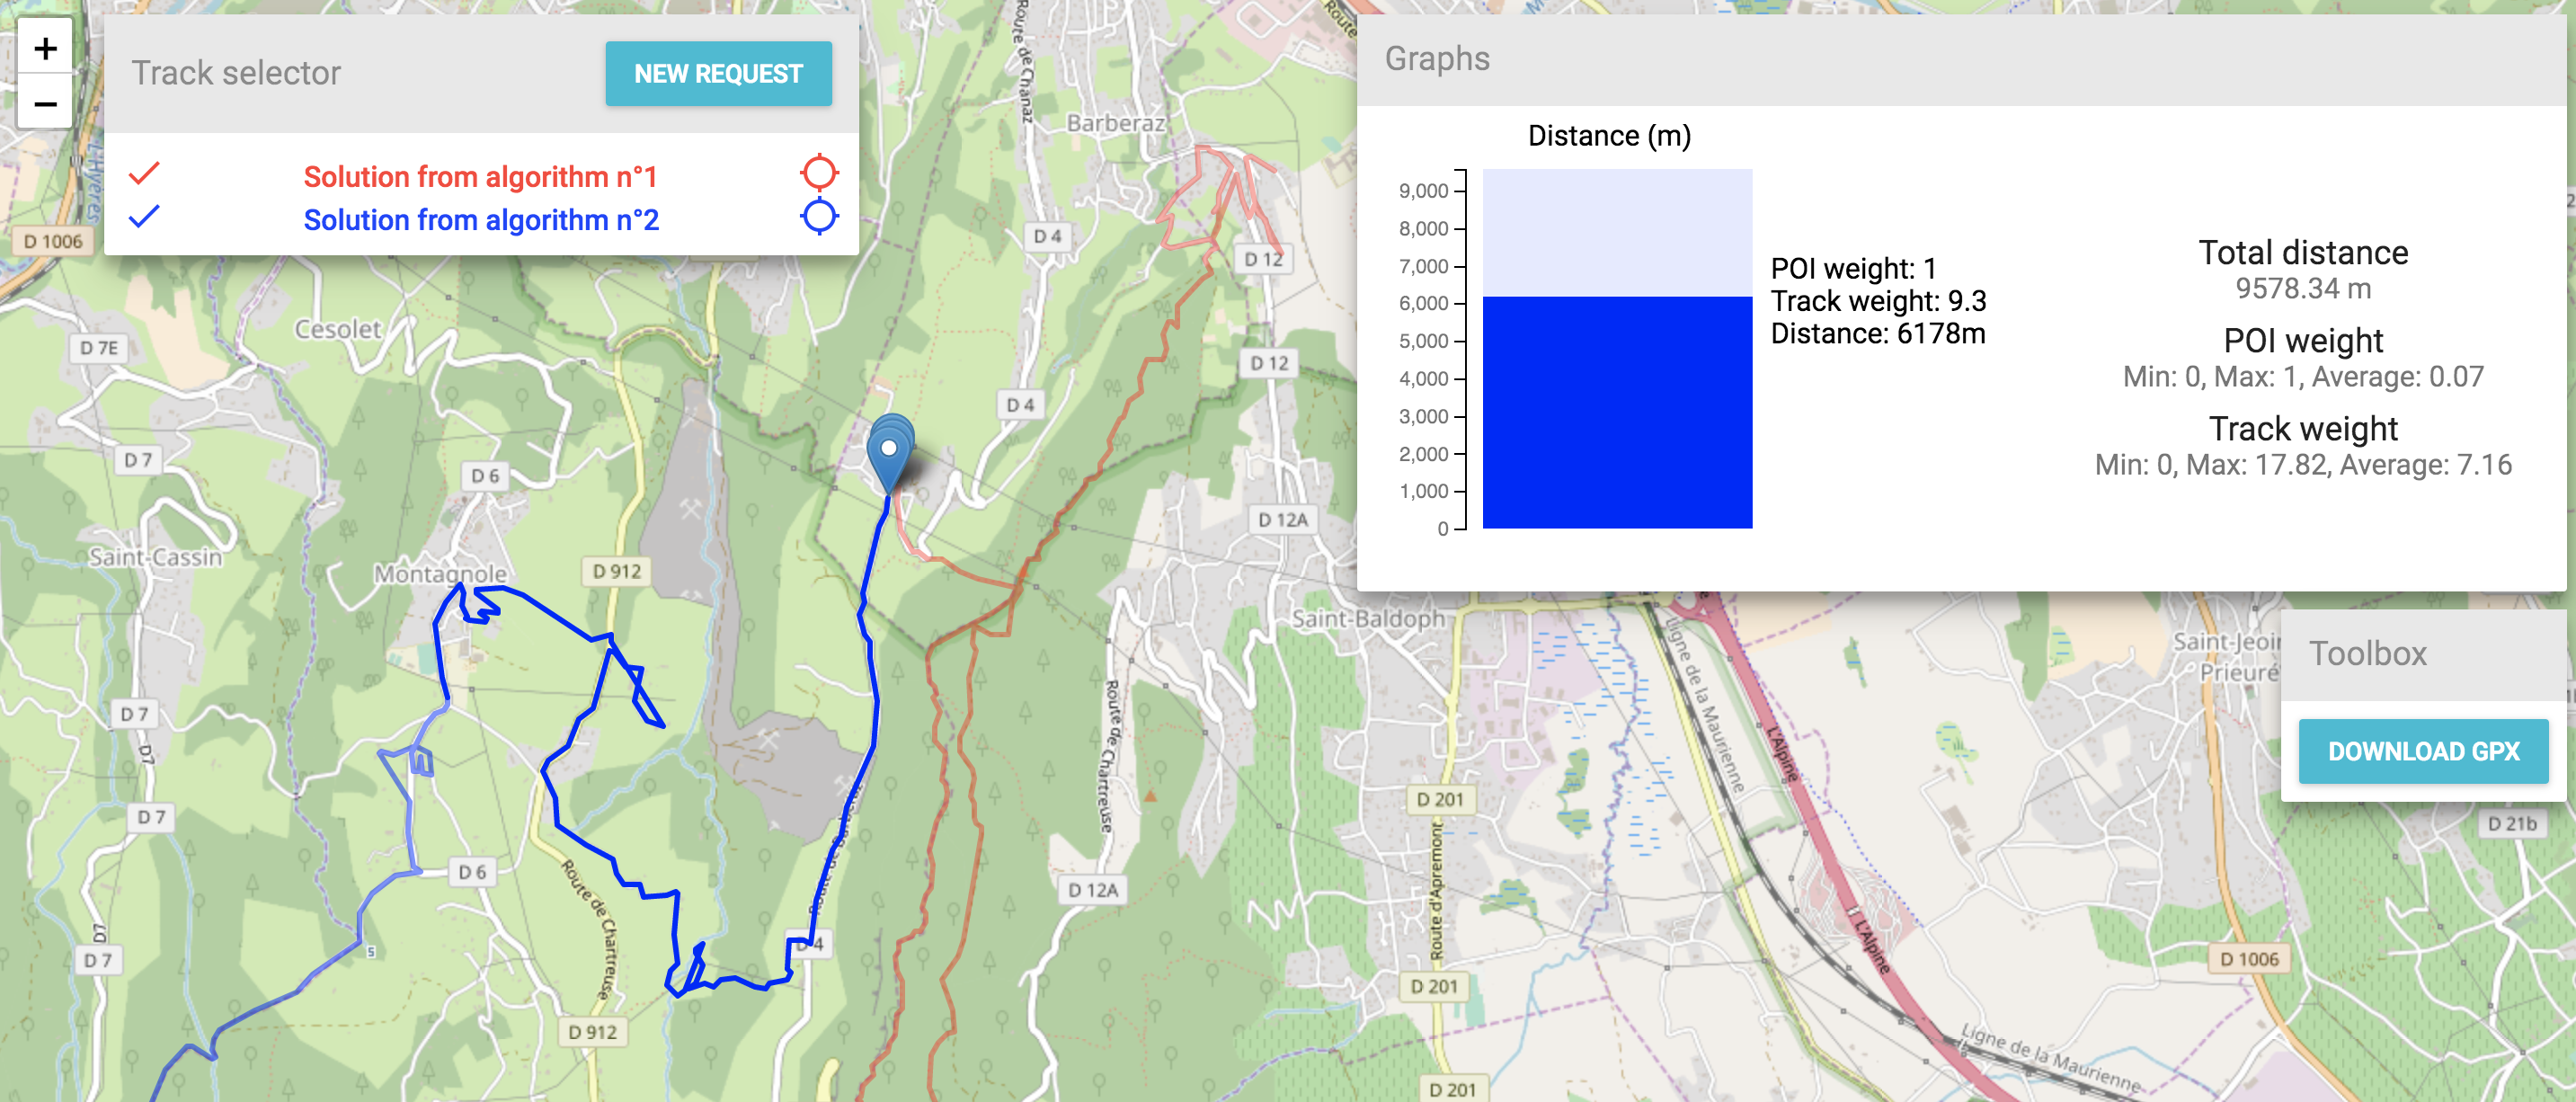
\includegraphics[width=\textwidth]{ux.png}
  \caption{UX interface, displaying some results}
  \label{figure:ux}
\end{figure*}

Finally, we used a library called Redux combined with React. This is a powerful method to deal with a unique "state" for our application and then distribute the state to every React component. Thus, data are centralized and can be easily updated.

\section{Evaluation of the solution}

\subsection{Experiments and evaluation}

To assess the performance of our approach and its possible added value, we tested it against two baselines: Google Maps and Utagawa. As shown in greater details in table \ref{table:baselines} on page \pageref{table:baselines}, our solution performs better than Google Maps and Utagawa in regards to POI proximity.

Utagawa is better at proposing paths that follow traditional trails, which is to be expected seeing that Utagawa consists entirely of those trails while our implementation and Google Maps contain non-trails as well. However, our implementation does perform better in this regard than Google Maps does.


\begin{table}
    \begin{tabular}{|lrr|} 
        \hline
        & Avg. POI weight & Avg. track weight \\
        &  per point & per point \\ 
        \hline
        Random point & under 0.001 & 0.055 \\ 
        Google Maps* & under 0.001 & 0.062 \\
        Utagawa** & 0.09 & \textbf{1.24} \\
        Our algorithm & \textbf{0.012} & 0.87 \\
        \hline
    \end{tabular}
    \captionsetup{justification=centering}
    \caption{Comparison against Google Maps\\ 
    * Random start and arrival locations points \\
    ** Not correlated with start location}
    \label{table:baselines}
    \end{table}

These values may seem low, but they were computed based on a large sample of roads and trails in and around Chamb\'{e}ry, France. Parts of this area had few Utagawa trails and POI, which lead to a decrease in the average track and POI weight values. Paths that started in areas saturated with Utagawa trails and POI tended to have larger POI and trail weights. This suggests that our implementation should perform very well in its ideal use case. 
    
Finally, the confusion matrix detailed in table \ref{table:confusion_matrix} on page \pageref{table:confusion_matrix} highlights that our algorithm only keeps the best tracks. This sort of analysis was suggested by Provost and Fawcett for finding ideal models (2013). For 409 generated tracks, only 5 were predicted as good according to the previously outlined method. Among these 5 tracks, none were false positives. Therefore, only top tracks are proposed to the user. However, this involves a big waste as a manual exploration (by arbitrary setting a trail weight mean of 5 and at least 2 POI per kilometer) of the predicted bad trails showed that many would have eventually become good trails and thus false negatives.

This algorithm ideally should satisfies our users and not wastes their time by only proposing the highest quality trails. However, our solution should be improved to reduce the number of false negatives, which would offer users more choices and not waste running time, which is directly tied to costs.

\begin{table}
    \begin{tabular}{|lrr|} 
         \hline
         & Good track & Bad track \\
         \hline
         Predicted good track & 5 & 0
         \\
         Predicted bad track & 135 & 269
         \\
         \hline
    \end{tabular}
    \captionsetup{justification=centering}
    \caption{Confusion matrix.}
    \label{table:confusion_matrix}
\end{table}

\subsection{Possible improvements}

The final solution works, but it could be easily improved with more time and data.

First, regarding the data, our implementation was limited to France because of limited websites for finding POI and trails. We also decided to limit ourselves to the area around Chamb\'{e}ry because of familiarity with the area and insufficient resources. Acquiring more data could be done through the official OpenStreetMap API or by downloading portions of the map through services like MapZen Metro Extract. However, this data takes up a lot of space and requires a long time to process.

As for integrating additional information, we tried to add for instance elevation and trail quality to our application, but this information was not included in OpenStreetMap data and needed to be queries from a service like Google Maps Elevation API. This API in particular imposed rate and query limits which would make it unfeasible for us to gather information for all of our data. It would have taken several years for the area we chose due to the 10,000 query limit of the API.

The UI could also be improved to include tons of features particularly useful for users such as the visualization of POI data or a mechanism that allow hikers to manually edit paths if they want to pass by a certain location.

We should also implement a feedback system to let hikers update the trail paths themselves and tell how they feel with a particular path. This data would help us to refine our results and to take into account trail changes. Additionally, establishing a pipeline from Utagawa to our application would further distinguish which paths are good and bad.

Finally, our algorithm first needs to gather the data from the map in a certain area around the begin location. Basically, it requests every points and road of the map in a radius equal of the maximum distance asked by the user, around the input begin location. This process can take a long time and increases with a power of two of the maximum distance. This data is then used to create the processing graph and search for the best paths. One possible solution could be to use more powerful servers; the program was only tested on our personal computers. Another is to restrict the amount of data gathered from the map, for instance by removing entire areas which are identified as useless and then not requested without impacting the relevance of solutions.

\section{Conclusion}
This project provides a simple and intuitive tool for producing interesting trails for bikers and hikers. While the application is not as efficient as we would like it to be, it has shown that it is feasible to construct a simple routing tool using only consumer grade hardware. More importantly, it shows that these tools can outperform consumer products in certain respects. The strength of our application is that it utilizes domain-specific information in ways that general-use products like Google Maps do not. Additionally, our methods were general enough that they could be used for other domain-specific mapping tools as well. For example, our algorithm outlined above could easily work for city-specific tourism and sightseeing. 

\subsection{Our group}
The TrailBlazer group was comprised of four M.S. students from the Georgia Institute of Technology with different educational and cultural backgrounds and this was an asset to success with this project. The work was split evenly among the team members. We managed to be efficient with different majors (mechanical engineering and computer science) and different nationality (American, French and Chinese).

% If a data pipeline from sources like Utagawa and geocaching.com could be established, then the quality of our generated paths would 

% it could further increase the quality of our trails. 

\subsection{About the project}
The total cost of the project was \textdollar 5, which covered the cost of hosting a database on MongoDB's Atlas service. As for timing, we accomplished as much as we could in the time allotted. Although there are areas for improvement, we are satisfied with the application we were able to build.
% \subsubsection{What we learned}

% Learned to work in group bla bla bla american stuff (github, drive, meeting, ...)

% Respect of the planning ?

% Experiment with powerful and modern tools : Django, React, ...
% This project was a great oportunity for us to work with several powe

% Dialogue with a frond end and a back end + remote database

\subsection{Future of the project}

TrailBlazer is still in an early stage but its algorithm and the UX interaction between the system and the user are tested and functional. The project is open source as are all of the libraries we used to build it. Some documentation is included, especially concerning installation and development and this present report and the previous ones can help too.

The entire code is on the open source website GitHub. Thus, anyone can improve the code or include it into another project freely.

\begin{thebibliography}{9}
\bibitem{} 
Agarwal, Sathak and KS Rajan. 
\textit{Analyzing the performance of NoSQL vs. SQL databases for Spatial and Aggregate queries.}. 
Free and Open Source Software for Geospatial Conference Proceedings 17, 2017.
 
\bibitem{} 
Allahbakhsh, Mohammad, Boualem Benatallah, and Aleksandar Ignjatovic.
\textit{Quality Control in Crowdsourcing Systems.}.
Web-Scale Workflow, 76-81, 2013.

\bibitem{} 
Amirian, Pouria, Anahid Basiri, and Adam Winstanley.
\textit{Evaluation of data management systems for geospatial big data}.
International Conference on Computational Science and Its Applications. Springer, Cham, 2014.

\bibitem{} 
Dijkstra, Edsger W.
\textit{A note on two problems in connexion with graphs}.
Numerische mathematik 1.1 (1959): 269-271.

\bibitem{} 
Fielding, Roy Thomas.
\textit{Architectural Styles and the Design of Network-based Software Architectures}.
Doctoral Dissertation, University of California, Irvine, 2000.

\bibitem{} 
Johnson, Donald B.
\textit{Finding all the elementary circuits of a directed graph}.
SIAM Journal on Computing 4.1 (1975): 77-84.

\bibitem{} 
Haklay, Mordechai.
\textit{How good is volunteered geographical information? A comparative study of OpenStreetMap and Ordnance Survey datasets}.
Environment and Planning B: Planning and Design 37 (2010): 682-703.

\bibitem{} 
Holte, Robert C.
\textit{Very Simple Classification Rules Perform Well on Most Commonly Used Datasets}.
Computer Science Department, University of Ottawa, 1993.

\bibitem{} 
Provost, Foster, and Tom Fawcett.
\textit{Chapter 7: Decision Analytic Thinking I: What Is a Good Model?}
Data Science for Business: What You Need to Know about Data Mining and Data-Analytic Thinking, O'Reilly (2013).

\bibitem{} 
Samer Buna.
\textit{All the fundamental React.js concepts}
Medium (blog), Aug 2017.
\\\texttt{goo.gl/LUMxtp}

\bibitem{} 
Provost, Foster, and Tom Fawcett.
\textit{Chapter 8: Visualizing Model Performance?}
Data Science for Business: What You Need to Know about Data Mining and Data-Analytic Thinking, O'Reilly (2013).

\bibitem{} 
Rosenzweig, Elizabeth.
\textit{Successful User Experience: Strategies and Roadmaps}.
Elsevier Science (2015): Chapter 3.

\bibitem{} 
Colt, Pini.
\textit{React + Redux: Architecture Overview}
Medium, Nov 2016.
\\\texttt{goo.gl/8xYN6Q}

\bibitem{} 
Tarjan, Robert.
\textit{Depth-first search and linear graph algorithms}.
SIAM journal on computing 1.2 (1972): 146-160.

% \bibitem{} 
% Paris, Michel.
% \textit{REST 2.0 is here and it’s name is GraphQL}
% SitePoint (blog), May 17, 2017.
% \\\texttt{https://www.sitepoint.com/rest-2-0-graphql/}

\bibitem{}
C. M., Thomas and W. E.,Featherstone.
Journal of Surveying Engineering, February 2005.
\textit{Validation of Vincenty’s Formulas for the Geodesic Using
a New Fourth-Order Extension of Kivioja’s Formula}

\bibitem{}
Alexandre PALO, Alex MUELLER, Tianyi ZHENG, Guillaume BROGGI.
\\\textit{TrailBlazer code and documentation}
\\\texttt{https://github.com/AlexandrePalo/TrailBlazer}

\bibitem{}
Groundspeak, Inc.
\\\textit{Geocaching website}
\\\texttt{https://www.geocaching.com}

\bibitem{}
Hukosai VTT association.
\\\textit{Utagawa VTT website}
\\\texttt{https://www.utagawavtt.com}

\bibitem{}
Mapzen
\\\textit{Mapzen website}
\\texttt{https://mapzen.com/}

\bibitem{}
Wing, Michael G., Aaron Eklund, Loren D. Kellogg.
\textit{Consumer-Grade Global Positioning System (GPS) Accuracy and Reliability}. 
Journal of Forestry 103. (2005): 169-173.
\end{thebibliography}

\end{document}
